\chapter{Fast One-Ring Smoothing}
In this chapter we present an updated version of the Fast One-Ring smoothing filter for scalar fields on discrete manifolds, based on the initially proposed by H. Mara and S. Krömker at the EUROGRAPHICS Workshop on Graphics and Cultural Heritage (2017) ~\cite[s.~3.2]{Mara17}. Since its publication, further research has been conducted by the authors and it was determined that the weighting methods required improvement, therefore, modifcations were made directly to the algorithm implemented within the GigaMesh \todoCitation framework. We will now present this as-yet-unpublished version of the Fast One-Ring smoothing filter as it exists now, with more accuracte weighting.
%
\section{Points \& Edges}
Given a point $\bp_0$ in a discrete manifold $\mathcal{M}$ which is comprised of $v$ number of points, the one-ring neighborhood $\mathcal{N}$ can be defined as all the points $\bp_i$ which share an edge with $\bp_0$, where $i \in \{1, \ldots, n\}$, and $n$ is the number of points in $\mathcal{N}$ which are always indexed in a clockwise direction\todoResearch{GigaMesh assumes a counter-clockwise direction}. The value of $n$ may vary among vertices in $\mathcal{M}$, however the value must always be $\geq 2$ and typically $\leq 12$, though there is no upper limit\todoResearch{get real upper limit for n}.%
\nomenclature{$\bp$}{a point in $\mathcal{M}$}%
\nomenclature{$\bp_0$}{the center point of $\mathcal{N}$}%
\nomenclature{$\bp_i$}{a one-ring neighbor of $\bp_0$}%
\nomenclature{$\mathcal{M}$}{a discrete manifold}%
\nomenclature{$v$}{number of points (vertices) in $\mathcal{M}$}%
\nomenclature{$\mathcal{N}$}{a one-ring neighborhood}%
\nomenclature{$n$}{the number of points in $\mathcal{N}$}%

The smallest edge length in the one-ring neighborhood $\mathcal{N}$ is 
\begin{equation}
	\Dm(\bp_0) := \text{min}^n_{i=1} (|\bp_i - \bp_0|)
	\label{eq:localMinimumEdgeLength}
\end{equation}
Abbreviated as $\Dm$, this length will be used as the radius of a geodesic disc on $\mathcal{M}$. \todoCitation{geodesic discs} Furthermore, to ensure that the filter remains the same size for all neighborhoods $\mathcal{N}$ in mesh $\mathcal{M}$, we define
\begin{equation}
	\overline{\Delta_\text{min}} := \min\{\Delta_\text{min}(\bp_0) \;|\; \bp_0 \in \mathcal{M}\}
	\label{eq:globalMinimumEdgeLength}
\end{equation} 
as the global shortest edge length, for all edges of the mesh. We will then use this $\overline{\Delta_\text{min}}$ in all the following computations. \todoReword{rewrite all Dms as globalDms}

Figure~\ref{fig:geodesicDisc} shows a typical configuration of an one-ring with irregular faces, the geodesic disc with radius 
$\Dm$, and circular sectors $\bs_i$ used for weighting.
\begin{figure}[ht]
\ffigbox
	{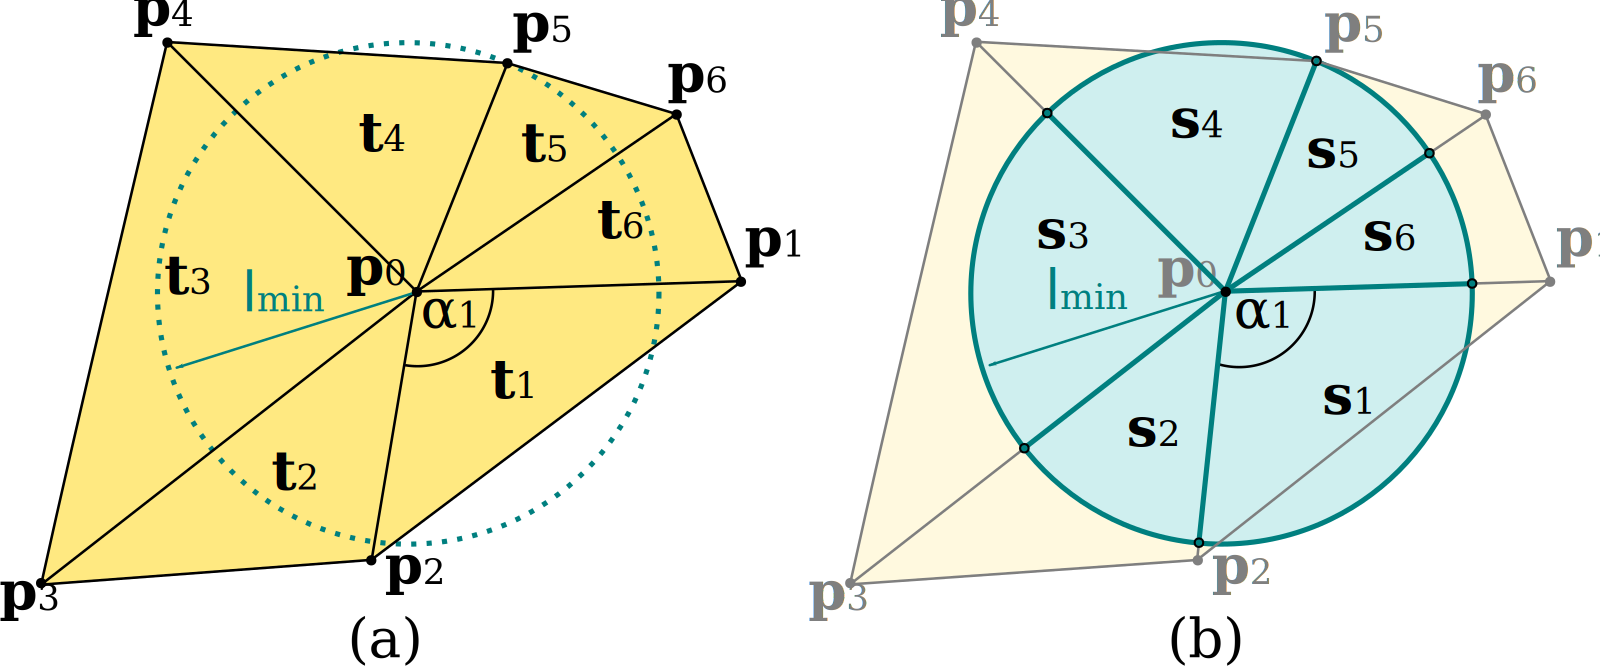
\includegraphics[width=0.5\linewidth]{figures/geodesicDisc.png}}
	{\caption[One-ring and geodesic disc]{A typical one-ring neighborhood $\mathcal{N}$ with (a) irregular triangular faces $\mathbf{t}_i$, the smallest edge length $\Dm = |\bp_4 - \bp_0|$ shown here with a cyan arrow as the radius of the geodesic disc, and $\alpha_i$ as the central angle of $\mathbf{t}_i$ (b) the complete geodesic disc, comprised of all its circular sectors $\bs_i$, each having central angles $\alpha_i$}\label{fig:geodesicDisc}}
\end{figure}%
\nomenclature{$\bs_i$}{circular sectors which comprise the geodesic disc}%

%
\section{Angles}
Because the angles $\alpha_i$ will be used in future calculations, but are not typically measured directly as are the edge lengths, it is worth mentioning that one can calculate an inner angle $\alpha_i$ using the law of cosines. \todoCitation{law of cosines}
\begin{equation}
	\alpha_i = cos^{-1}(\frac{|\bp_0 - \bp_{i}|^2 + |\bp_0 - \bp_{\sipo}|^2 - |\bp_i - \bp_{\sipo}|^2}{2\cdot|\bp_0 - \bp_{i}|\cdot|\bp_0 - \bp_{\sipo}|})
	\label{eq:alphaFromEdgeLengths}
\end{equation}

For interpolation of the function values over the entire circular sector, we must first interpolate the values one side of the bisecting line at a time. The angles $\beta_i$ are therefore calculated using the third angle theorem as the third angle to form a right triangle along with $\alpha_i/2$ for each half of $\bs_i$. \todoCitation{and third angle theorems}
\begin{equation}
	\beta_i = \Big(\frac{\pi}{2} - \frac{\alpha_i}{2}\Big) = \frac{(\pi - \alpha_i)}{2}
	\label{eq:betaFromHalfAlpha}
\end{equation}
%
\section{Area \& Center of Gravity (centroid)} 
We also need the area of each circular sector $\bs_i$ comprising the geodesic disc of $\mathcal{N}$, which can be calculated with just $\Dm$ and $\alpha_i$
\begin{equation}
	A_i = \frac{(\Dm)^2\alpha_i}{2}
	\label{eq:circularSectorArea}
\end{equation}
\todoCitation{area of circle sectors, http://mathworld.wolfram.com/CircularSector.html}%
\nomenclature{$A_i$}{area of circular sector $i$}%

Next, the distance from the center point $\bp_0$ to the center of gravity for the circular sector $\bs_i$ is calculated as
\begin{equation}
	\Dc_i := \frac{2\:\Dm\:\sin(\frac{\alpha_i}{2})}{3\:\frac{\alpha_i}{2}}
	\label{eq:distToCoG}
\end{equation}
\todoCitation{area of circle sectors, http://mathworld.wolfram.com/CircularSector.html}%
\nomenclature{$\Dc_i$}{the distance to the center of gravity $\bc_i$ within circle sector $\bs_i$}%

Figure~\ref{fig:centerOfGravity} illustrates the center of gravity, or centroid, \todoCitation{centroid} and its distance from the center point of the circular sector, using $\bs_i$ from Figure~\ref{eq:localMinimumEdgeLength} as an example. In general, the smaller the angle $\alpha_i$ of the circle sector, the longer the distance $\Dc_1$ becomes.
\begin{figure}[ht]
\ffigbox
	{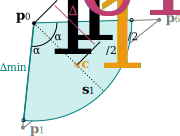
\includegraphics[width=0.6\linewidth]{figures/centerOfGravity.png}}
	{\caption[Distance to and Center of Gravity]{A single circle sector $\bs_1$ with a bisecting line in black dots and its center of gravity $\bc_1$ marked in a sand color, as well as the distance from the center point $\bp_0$ to $\bc_1$ drawn in coral as $\Dc_1$}\label{fig:centerOfGravity}}
\end{figure}%
\nomenclature{$\bs_i$}{circular sectors which comprise the geodesic disc}%
%
\section{Interpolation}
With $\alpha_i/2$, $\beta_i$, and $\Dm$ being constant for both halves of any circular sector $\bs_i$ , we can next use the Law of Sines to obtain a constant ratio by which we can interpolate the three function values at the points $\bp_0$, $\bp_i$, and $\bp_{\sipo}$ which comprise the face $\mathbf{t}_i$.
\begin{equation}
	\zeta_i = \frac{\Dm}{\sin(\beta_i)}
	\label{eq:zeta}
\end{equation}

With the constant ratio $\zeta_i$, we can obtain both of the distances for interpolation. Please note, because the points $\bp_i$ and $\bp_{\sipo}$ are likely at different distances from the center point $\bp_0$, we must now begin calculating for each half of the circular sector individually, therefore we  adopt the subscript to denote the index of the sector, as in $\bs_i$, and the superscript to denote the side of the sector defined by its point, as in $\zeta^{\sipo}$ is used with $\bp_{\sipo}$.
\begin{align}
	\zeta^i_i & = \enspace\frac{\zeta_i}{|\bp_0 - \bp_i|}
	\label{eq:distanceIForInterpolation}\\
	\zeta^{\sipo}_i & = \frac{\zeta_i}{|\bp_0 - \bp_{\sipo}|}
	\label{eq:distanceIp1ForInterpolation}
\end{align}
\todoReword{every equation needs a nomenclature entry}

From the original function values $f_0$, $f_i$, and $f_{\sipo}$, we can now interpolate based on their distances $\zeta^i_i$ and $\zeta^{\sipo}_i$, to become
\begin{align}
	f^{'i}_i & = f_0(1 - \zeta^i_i) + f_i\zeta^i_i \\
	f^{'\sipo}_i & = f_0(1 - \zeta^{\sipo}_i) + f_{\sipo}\zeta^{\sipo}_i
	\label{eq:interpolatedFs}
\end{align}
%
\section{Weighted Mean}
To calculate the weighted mean function value $f^\bs_i$ at the center of gravity $\bc_i$ of the circle sector $\bs_i$, we must use the function value at $\bp_0$, both interpolated function values $f^{'i}_i$ and $f^{'\sipo}_i$, and the distance to the center of gravity $\Dc_i$, and we obtain
\begin{equation}
	f^\bs_i = f_0(1 - \Dc_i) + \frac{(f^{'i}_i + f^{'\sipo}_i)\Dc_i}{2};
	\label{eq:weightedMeanAtCoGatSector}
\end{equation}

Finally, we can compute the one-ring weighted mean function value at $\bp_0$ by summing all the weighted mean function values from each $\bs_i$ in $\mathcal{N}$, weighting those again by each sector's area $A_i$, then finally dividing by the total area of the geodesic disc.
\begin{equation}
	\bar{f}_0 := \frac{\sum A_if^{\bs}_i}{\sum A_i} \quad \forall i \in \{1,\ldots,n\}
	\label{eq:meanFuncValAtP0}
\end{equation}%
\nomenclature{$\bar{f}_0$}{the one-ring weighted mean function value at $\bp_0$}%

The one-ring smoothing filter can be modified to use the median operation, instead of the mean, by using all the equations except ~\ref{eq:meanFuncValAtP0} and then sorting the results of ~\ref{eq:weightedMeanAtCoGatSector}. The details of which can be found by the original publication ~\cite[s.~3.2]{Mara17}, but as it was not implemented in GPGPU for this thesis, we exclude the details here. 
%
\section{Summary}
In this chapter we presented an updated version of the Fast One-Ring smoothing filter for scalar fields on discrete manifolds, which since its original publication ~\cite[s.~3.2]{Mara17}, now utilizes the entire area of the geodesic disc $A$ for calculating the weighted averages. First, we have illustrated how one can calculate the smallest edge length $\Dm$, interior angles $\alpha$ and $\beta$, the area $A$ of a sector $\bs$ from the geodesic disc, and distance to the centroid (center of gravity) $\Dc$ for any given one-ring neighborhood $\mathcal{N}$. Next, we provided the equations for interpolating the three function values $f_0$, $f_i$, and $f_{\sipo}$ using the constant ratio $\zeta$ to obtain the weighted mean function value for each $\bs$, and finally the weighted mean function value $\bar{f_0}$ at point ${\bp_0}$ for the entire one-ring neighborhood $\mathcal{N}$. Convolving this filter with the scalar field of function values at each vertex in a mesh, thus produces a smoothing effect. 






